\documentclass[12pt]{report}
\usepackage{etex}
\usepackage{amsmath,amsxtra,amssymb,latexsym,amscd,amsthm}
\usepackage{indentfirst}
\usepackage{epigraph}
\usepackage{tabvar}
\usepackage{ifpdf}
\usepackage[english]{babel}
\usepackage[mathscr]{eucal}
\usepackage{graphics, graphicx}
\usepackage{pstricks,pst-node,pst-tree}
\usepackage{caption}
\usepackage{subcaption}
\usepackage{fancybox}
\usepackage[colorlinks=true]{hyperref}  
\usepackage[a4paper,left=15mm,right=10mm,top=15mm,bottom=15mm]{geometry}
\renewcommand{\baselinestretch}{1.5}
\usepackage{fancyhdr}
\usepackage{pifont}
\usepackage[mathscr]{eucal}
\usepackage{wrapfig}
\usepackage{tikz}
\usetikzlibrary{arrows}
\renewcommand{\qedsymbol}{\ding{114}}
\newcommand{\h}{$\bigotimes$ }
\newcommand{\tl}{$\bigodot$ }
\newcommand{\het}{ \begin{flushright} \ding{114} \end{flushright}}

\def\lc{\left\lceil}   
\def\rc{\right\rceil}
\newcommand{\td}{$ \Leftrightarrow $ }
\newcommand{\sr}{\Rightarrow }
\newcommand{\sao}{$\divideontimes$ }
\newcommand{\lf}{\left (}
\newcommand{\ri}{\right )}
\newcommand{\co}{\texttt}
\usepackage{listings}
\usepackage{color}



\definecolor{dkgreen}{rgb}{0,0.6,0}
\definecolor{gray}{rgb}{0.5,0.5,0.5}
\definecolor{mauve}{rgb}{0.58,0,0.82}

\lstset{
  backgroundcolor = \color{white},
  frame=tb,
  language=Java,
  aboveskip=3mm,
  belowskip=3mm,
  showstringspaces=false,
  columns=flexible,
  basicstyle={\small\ttfamily},
  numbers=none,
  numberstyle=\tiny\color{gray},
  keywordstyle=\color{blue},
  otherkeywords = {var, func, let},
  commentstyle=\color{red},
  stringstyle=\color{mauve},
  breaklines=true,
  breakatwhitespace=true,
  tabsize=3
}

\begin{document}
\tableofcontents
\newpage
\chapter{Basic syntax}
\section{Variables}
Variables are declared as
\begin{lstlisting}
[strong/ weak] var [variable-name] : [variable-type] [? / !]
\end{lstlisting}
Optional variables marked with ? are \co{optional}.\\
Variables have to be initialized upon declaration. Optional variables are automatically initialized as \co{nil}. \\
Declare optional type as ! rather than ? means automatic unwrap (so don't have to add ! every time we want to unwrap). \\
Computed property:
\begin{lstlisting}
	var displayValue : Double {
		get {
			return NSNumberFormatter().numberFromString(display.text!)!.doubleValue;
		}
		set {
			// newValue is by default the new value that displayValue is set to
			display.text = "\(newValue)" // convert stuff into String
		}
	}
\end{lstlisting}

\section{Functions}
Functions are declared as
\begin{lstlisting}
func [function[name] ([param 1 name] : [param 1 type], ... )
\end{lstlisting}
Pass function type as parameter type:
\begin{lstlisting}
	func performOperation(operation: (Double, Double) -> Double) {
		var result = operation(..., ...)
	}
	// FIRST WAY TO CALL performOperation
	func multiply(op1: Double, op2: Double) -> Double {
		return op1 * op2
	}
	performOperation(multiply)
	
	// SECOND WAY TO CALL performOperation
	performOperation({ (op1: Double, op2: Double) -> Double in 
		return op1 * op2
	})
	
	// THIRD WAY TO CALL performOperation (use type inference)
	performOperation({ (op1, op2)  in 
		 op1 * op2 // return keyword is optional
	})
	
	// 4TH WAY TO CALL performOperation
	performOperation({ 
		 \$0 * \$1 // does not need to specify parameter name
	})
	
	// MOST CONCISE WAY
	performOperation { \$0 * \$1} // function as last argument can be declared outside of ( ). if no other argument, () can also be omitted
\end{lstlisting}
Constructors are called \co{init()}.

\section{Basic data structures}
\subsection{Array}
$$\co{var operandStack : Array<Double> = Array<Double>()} $$
Note that type can be omitted because Swift has type inference.\\
Alternative and preferred: \co{[Double]()}. \\
Array is a \co{struct}.

\subsection{Dictionary}
$$\co{var knownOps = Dictionary<String, Op>()}$$
Alternative and preferred: \co{[String : Op]()}. 
Dictionary is a \co{struct}. Enumerate Dictionary using tuples:
\begin{lstlisting}
pacl10teamRankings = ["Stanford" : 1, "Cal": 10]
let ranking = pacl10teamRankings["Ohio State"]
for (key,value) in pack10teamRankings {
	println("\(key) = \(value)")
}
\end{lstlisting}

\subsection{Range}
Two end points of a sensible type.
\begin{lstlisting}
struct Range<T>{
	var startIndex: T
	var endIndex: T
}
\end{lstlisting}
Specifying a Range:
\begin{lstlisting}
let array = ["a", "b", "c", "d"]
let subArray1 = array[2..3] // 2 to 3 inclusive
let subArray2 = array[2..<3] // 2 to 3 not including 3
for i in [27..104] {

}
\end{lstlisting}

\section{Enum}
Can have functions. Only computed properties.
\begin{lstlisting}
enum Op{
	case Operand(Double)
	case UnaryOperation(String, Double -> Double)
	case BinaryOperation(String, (Double, Double) -> Double)
}

var opStack = [Op]()
var knownOps = [String, Op]()

func pushOperand(operand: Double){
	opStack.append(Op.Operand(operand))
}

func performOperation(symbol: String){
	// let operation = ..., if operation != nil ... 
	if let operation = knownOps[symbol] { 
		opStack.append(operation)
	}
}

func evaluate() -> Double? {
	
}
\end{lstlisting}

\chapter{Other language-specific notes}

\section{Private vs Public}
\begin{itemize}
\item If no keyword \co{private}, variables are public inside your program. Only use \co{public} when you ship a framework.
\end{itemize}

\section{Value vs Reference}
\begin{itemize}
\item \co{struct} does not have inheritance and, like \co{enum}, is passed by value, not reference. There's an implicit \co{let} in front of parameter declaration, so parameters passed by value are immutable.(can specify \co{var}).
\item Function parameters are by default constants. You can put the keyword \co{var} on an parameter, and it will be mutable, but it's still a copy.
\item You must note any function that can mutate a struct/enum with the keyword \co{mutating}.
\item Constant pointers to a class (\co{let}) still can mutate by calling methods and changing properties.
\end{itemize}

\section{Methods}
\begin{itemize}
\item All parameters to all functions have {\bf internal} name and an {\bf external} name. The internal name is the local variable you use inside the method. The external name is what callers will use to call the method.
\begin{lstlisting}
	func foo(external internal: Int){
		let local = internal
	}
	func bar(){
		let result = foo(external: 123)
	}
\end{lstlisting}
\item You a use bar to specify "dont' care". 
\begin{lstlisting}
	func foo(_ internal: Int){
		let local = internal
	}
	func bar(){
		let result = foo(123)
	}
\end{lstlisting}
\item The bar is default for the first parameter (only) in a method, but not for \co{init} methods. You can force the first parameter's external name to be the internal name with \co{\#}. For other (not the first) parameters, the internal name is by default the external name.
\end{itemize}

\section{Properties}
\begin{itemize}
	\item You can observe any changes to any property with \co{willSet} and \co{didSet}. One very commong thing to do in an observer in a Controller is to update the user-interface.
	\begin{lstlisting}
		var someStoredProperty : Int = 42 {
			willSet { 
				//newValue is the new value
			}
			didSet {
				// oldValue is the old value
			}
		}
	\end{lstlisting}
	\item A lazy property does not get initialized
\end{itemize}

\section{Initializer}
\begin{itemize}
\item You can set any property's value, even those with default values. Constant properties declared with \co{let} can also be set.
\item By the time any \co{init} is done, all properties must have values (optionals can have the value \co{nil}).
\item You must initialize all properties introduced by your class before calling a superclass's \co{init}.
\item You must call a superclass's \co{init} before you assign a value to an inherited property.
\item A designated init can only call a desginated init in its immediate subclass.
\item A class can mark one or more of its init methods as \co{required}. Any subclass must implement such init methods.
\end{itemize}

\subsection{Inheriting init}
\begin{itemize}
	\item If you do not implement any designated inits, you will inherit all of your superclass's designateds.
	\item If you override all of your superclass's designated inits, you will inherit all its convenience inits.
\end{itemize}

\subsection{Creating objects}
Create an object by calling it's initializer via the type name or by calling type methods in classes
\begin{lstlisting}
	let x = CalculatorBrain()
	let z = [String]()
	let button = UIButton.buttonWithType(UIButtonType.System)
\end{lstlisting}
Sometimes other objects will create objects for you.
\begin{lstlisting}
	let commaSeparatedArrayElements: String = ".".join(myArray)
\end{lstlisting}

\subsection{Conversion between types with \co{init()}}
\begin{lstlisting}
	let d: Double = 37.5
	let f: Float = 37.5
	let x = Int(d)		// truncates
	let xd = Double(x)
	let cgf = CGFloat(d)

	let a = Array("abc")
	let s = String(["a", "b", "c"])
	let s = "\(37.5)"
\end{lstlisting}


\section{Casting}
Casting is done using the keyword \co{as}.
\begin{lstlisting}
// crash if destinationViewController is not a CalculatorViewController
let calcVC = destinationViewController as CalculatorViewController
\end{lstlisting}

To protect against a craash, use \co{if let} with \co{as?}, which returns an optional.
\begin{lstlisting}
if let calcVC = destinationViewController as? CalculatorViewController { ... }
\end{lstlisting}

Or we can check the type.
\begin{lstlisting}
if destinationViewController is CalculatorViewController { ... }
\end{lstlisting}

Can also cast a whole array.
\begin{lstlisting}
var toolbarItems: [AnyObject]
// first way
for item in toolbarItems {
	if let toolbarItems = item as? UIBarButtonItem {
		// do something
	}
}
// second way. note no ? here
for toolbarItem in toolbarItems as [UIBarButtonItem] { 
	// do something
}
\end{lstlisting}


\section{Useful functions}
\begin{itemize}
	\item Array: say \co{var arr = [a,b,c]}.
	\begin{lstlisting}
	+= [T] // add another array to the end
	first -> T? // optional
	last -> T? // optional
	append(T)
	insert(T, atIndex: Int)				// arr.insert(d, atIndex: 1) yields arr = [a,d,b,c]
	splice(Array<T>, atIndex: Int)		// arr.splice([d,e], atIndex: 1) yields arr = [a,d,e,b,c]
	removeAtIndex(Int)					// arr.removeAtIndex(1) yields arr = [a,c]
	removeRange(Range)					// arr.removeRange(0..<2) yields arr = [c]
	replaceRange(Rance, [T])			// arr.replaceRange(0..1, with: [x,y,z]) yields arr = [x,y,z,b]
	sort(isOrderedBefore:(T,T) -> Bool)	// arr.sort({$0 < $1})
	filter(includeElement: (T) -> Bool) -> [T] // if includeElement returns false, T is removed
	map(transform:(T) -> U) -> [U]		// let stringified: [String] = [1,2,3].map{"\($0)"}
	reduce(initial: U, combine: (U,T) -> U) -> U // let sum: Int = [1,2,3].reduce(0) {$0 + $1}
	\end{lstlisting}
\end{itemize}

\section{String}
Substrings and indexes are all about the global \co{advance} function.
\begin{lstlisting}
	var s = "hello"
	let index = advance(s.startIndex, 2)	// index is a String.Index to the 3rd glyph, "l"
	s.splice("abc", index)					// s = "heabcllo"

	let startIndex = advance(s.startIndex, 1)
	let endIndex = advance(s.startIndex, 6)
	let substring = s[index..<endIndex] 	// substring will be "eabcl"

\end{lstlisting}

Use \co{Range} to get substring.
\begin{lstlisting}
let num = "56.25"
	if let decimalRange = num.rangeOfString(".") {	// decimalRange is Range<String.Index>
		let wholeNumberPart = num[num.startIndex..<decimalRange.startIndex]
	}
\end{lstlisting}

\section{Assertions}
Intentionally crash your program if some condition is not true (and give a message).
\begin{lstlisting}
assert(() -> Bool, "message")
assert(validation() != nil, "the validation functions returned nil")
\end{lstlisting}

\section{NSUserDefaults}
A Property List is a collection of objects which are ONLY one of $$\co{NSString, NSArray, NSDictionary, NSNumber, NSData, NSDate}$$
\co{NSUserDefaults} is a tiny database that stores Property List data, which persists between launchings of your application. Great for things like "settings" and such.
\begin{lstlisting}
	setObject(AnyObject, forKey: String)		// AnyObject must be a Property List
	objectForKey(String) -> AnyObject?
	arrayForKey(String) -> Array<AnyObject>?	// returns nil if value is not set or not an array

	setDouble(Double, forKey: String)
	doubleForKey(String) -> Double 				// not an optional, return 0 if no such key
\end{lstlisting}
Example code:
\begin{lstlisting}
	let defaults = NSUserDefaults.standardUserDefaults()
	let plist : AnyObject = defaults.objectForKey(String)

	// Be sure changes are saved at any time by synchronizing
	if !defaults.synchronize() {
		// failed, not much you can do about it
	}

\end{lstlisting}

\section{NSAttributedString}
\begin{lstlisting}
func setAttributes(attributes: Dictionary, range: NSRange)
func addAttributes(attributes: Dictionary, range: NSRange)
\end{lstlisting}
This is a pre-Swift API. \co{NSRange} is not a \co{Range}.\\
Attributes examples:
\begin{lstlisting}
NSForeGroundColorAttributeName : UIColor
NSStrokeWidthAttributeName : CGFloat
NSFontAttributeName : UIFont
\end{lstlisting}
To get the right font:
\begin{lstlisting}
preferredFrontForTextStyle(UIFontTextStyle) -> UIFont
// some of the styles
UIFontTextStyle.Headline
UIFontTextStyle.Body
UIFontTextStyle.Footnote
\end{lstlisting}



\chapter{View}
The top of the usable view hierarchy is the Controller's \co{var view: UIView}. This view is the one whose bound will change on rotation, and likely the one you will programmatically add subviews to.\\
Instead of initializing, you can call \co{awakeFromNib()} (only for views that come out of a storyboard).\\
\section{Coordinate system}
To work with view's coordinate system, use \co{CGFloat}. Double and Float can be converted to CGFloat by \co{let cfg = CGFloat(aDouble)}.\\
\co{CGRect} is a struct with a \co{CGPoint} and a \co{CGSize} in it.
\begin{lstlisting}
struct CGRect {
	var origin: CGPoint
	var size: CGSize
}
// convenient properties and functions
var minX: CGFloat				// left edge
var midY: CGFloat				// midpoint vertically
intersects(CGRect) -> Bool 		// intersection
intersect(CGRect)				// create an intersection of 2 CGRects
contains(CGPoint)  -> Bool 		// contain given point?
\end{lstlisting}
\co{var bounds: CGRect} is the rectangle containing the drawing space in its own coordinate system.\\
\co{var center: CGPoint} in the center of a \co{UIView} in its superview's coordinate system.\\
\co{var frame: CGRect} is the rect containing a \co{UIView} in its superview's coordinate system. \co{frame} is used for positioning, not drawing inside a view's coordinate system.\\
Views can be rotated, so \co{frame.size} is not equal to \co{bounds.size}. \\
By default, when a \co{UIView}'s bound changes, there is no redraw. Instead the bits of the existing images are scaled to the new bounds size. This is often not what you want, but there is a \co{UIVew} property to control this: $$\co{var contentMode: UIViewContentMode}$$
Or you can just call \co{.reDraw}.


\section{Creating views via code}
\begin{lstlisting}
	let labelRect = CGRect(x: 20, y: 20, width: 100, height: 50)
	let label = UILabel(frame: labelRect)
	label.text = "hello"
	view.addSubview(label)
\end{lstlisting}


\section{Custom views}
To draw a custom view, just create a \co{UIView} subclass and override \co{drawRect}: 
\begin{lstlisting}
override func drawRect(regionThatNeedsToBeDrawn: CGRect)
\end{lstlisting}
NEVER call \co{drawRect}. If your view needs to be redrawn, let the system know by calling 
\begin{lstlisting}
setNeedsDisplay()
setNeedsDisplay(regionThatNeedsToBeDrawn: CGRect)
\end{lstlisting}

\section{Drawing images}
\begin{lstlisting}
let image: UIImage = ...
image.drawAtPoint(aCGPoint)			// the upper left corner of the image put at CGPoint
image.drawInRect(aCGRect)			// scales the image to fit CGRect
image.drawAsPatternInRect(aCGRect)	// tiles the image into a CGRect
\end{lstlisting}


\chapter{Autolayout}
Example 1: Arrange grids so that:
\begin{itemize}
	\item All buttons have same size.
	\item Same spacing between neighbors and boundaries.
\end{itemize}
1st step:
\begin{center} 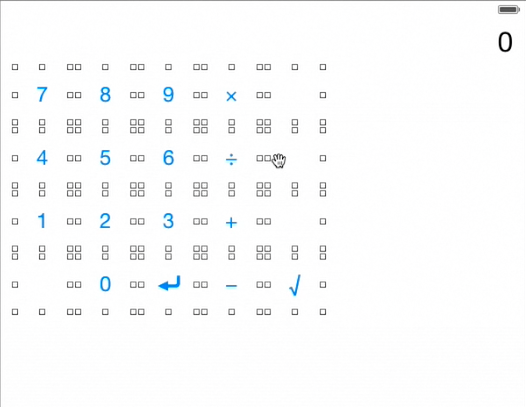
\includegraphics[scale = 0.5]{autolayout1.png} \end{center}
2nd step:
\begin{center} 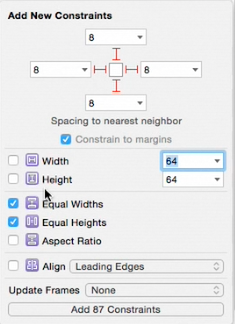
\includegraphics[scale = 0.5]{autolayout1_1.png} \end{center}
\end{document}